% Created 2018-07-11 Wed 15:45
% Intended LaTeX compiler: pdflatex
\documentclass[11pt]{article}
\usepackage[utf8]{inputenc}
\usepackage[T1]{fontenc}
\usepackage{graphicx}
\usepackage{grffile}
\usepackage{longtable}
\usepackage{wrapfig}
\usepackage{rotating}
\usepackage[normalem]{ulem}
\usepackage{amsmath}
\usepackage{textcomp}
\usepackage{amssymb}
\usepackage{capt-of}
\usepackage{hyperref}
\usepackage{placeins}
\usepackage[margin=0.5in]{geometry}
\usepackage[parfill]{parskip}
\date{\today}
\title{}
\hypersetup{
 pdfauthor={},
 pdftitle={},
 pdfkeywords={},
 pdfsubject={},
 pdfcreator={Emacs 26.0.91 (Org mode 9.1.13)}, 
 pdflang={English}}
\begin{document}

\tableofcontents

\section{Ressourcen, Prozesse und Ziele betrieblicher Leistungserstellung}
\label{sec:org5c6bc35}
\subsection{Leistungsbereich(Produktion)}
\label{sec:orgf19cd70}
\begin{center}
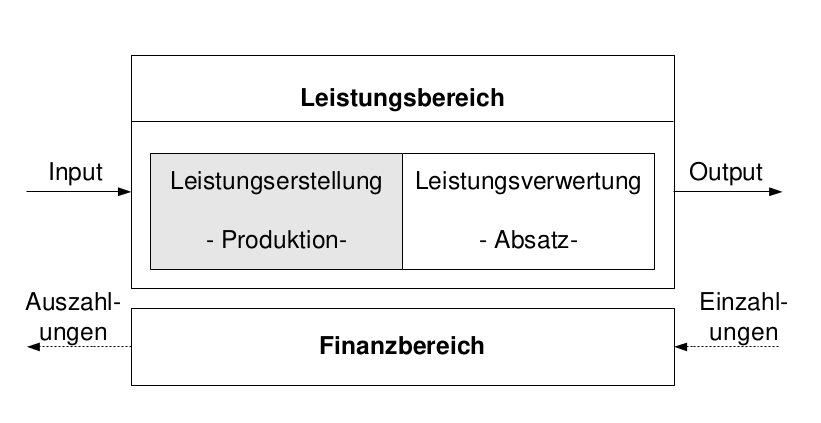
\includegraphics[width=250px]{./pictures/leistungsbereich_prod.png}
\end{center} 

\subsubsection{Produktion, Produktionsfaktoren, Produktionswirtschaft}
\label{sec:org8b4c66c}
\textbf{Produktion} = der industrielle Abbau von Material, dessen Be- und Verarbeitung und die Ausführung von Dienstleistungen; ist die methodische Umwandlung von Produktionsfaktoren in Produkte im Rahmen von bestimmten Produktionsverfahren

\textbf{Produktionsfaktoren} = sind die in der Produktion eingesetzen materiellen und immateriellen Güter, durch deren Gebrauch \& Verbrauch neue Sachgüter \& Dienstleistungen (Services) entsehen; Produktionsmittel nach Gutenberg = Betriebsmittel, Werkstoffe, (objektbezogene/dispositive) Arbeitsleistungen

\textbf{Produktionswirtschaft} = Aufgabe der Produktionswirtschaft ist die Planung, Durchführung \& Kontrolle der industriellen Leistungserstellung, um wirtschaftliche Produktionsstrukturen zu erreichen \& zu sichern
\subsection{Finanzierungsbereich}
\label{sec:org7f6506f}

\begin{center}
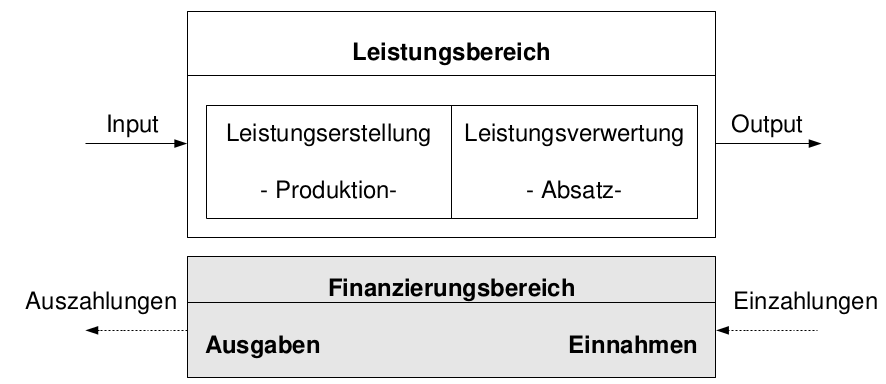
\includegraphics[width=250px]{./pictures/finanzierungsbereich.png}
\end{center} 

Finanzierung ist sowas wie eine Beanspruchung unter Versprechen auf Erfüllung
\begin{itemize}
\item betriebliche Finanzierung umfasst Beschaffung und Rückzahlung finanzieller Mittel und damit verbunden die Gestaltung der Beziehungen zw Unternehmen und Kapitalgebern
\item \emph{Finanzierungsmaßnahmen} beginnen mit Einzahlung an das Unternehmen, worauf Auszahlungen in späteren Perioden Folgen (Passivseite der Bilanz)
\item Gesamtheit aller Finanzmittel eines Unternehmens wird als Kapital bezeichnet
\end{itemize}

Investition ist sowas wie Verzicht in der Hoffnung auf Belohnung
\begin{itemize}
\item zielgerichteter Einsatz von finanziellen Mitteln zur Erwirtschaftung von Erträgen
\item \emph{Investitionsmaßnahmen} beginnen mit Auszahlung an das Unternehmen, auf die Einzahlungen in späteren Perioden folgen (Aktivseite der Bilanz)
\end{itemize}

\subsubsection{Finanzwirtschaft \& Zahlungsströme}
\label{sec:org76b690e}
\textbf{Monetärer Kapitalbegriff} = im Unternehmen eingesetzte Zahlungsmittel

\textbf{Finanzierung} ist die Kapitalbeschaffung für die jeweilige Unternehmung. Die \textbf{Finanzwirtschaft} umfasst diese Kapitalbeschaffung und -verwendung in der Unternehmung. Zu den finanzwirtschaftlichen Zielen gehört die Erreichung eines \emph{finanzwirtschaftlichen Gleichgewichts}, das bedeutet die Sicherung der dispositiven Liquidität, sowie die Sicherung der strukturellen Liquidität.

Die Funktion des \textbf{Finanzmanagements} ist die zielgerichtete Gestaltung der betrieblichen Finanzwirtschaft. Dazu zählt hauptsächlich die aktive Gestaltung der Kapitalzuführung \& des Kapitalentzugs.

\paragraph{Monetäre Zielgrößen}
\begin{itemize}
\item Zahlungsmittelbestand = Kassenbestand, Guthaben bei Kreditinstituren; Einzahlung, Auszahlung
\item Geldvermögen = Zahlungsmittelbestand + Forderungen - Verbindlichkeiten; Einnahme, Ausgabe
\item Gesamtvermögen = Gewinn + Verlustrechnung; Ertrag, Aufwand
\item Betriebsnotwendiges Vermögen = Kosten- und Leistungsrechnung; Ertrag, Aufwand
\end{itemize}

\section{Ressourcenbereitstellung \& Wettbewerbsfähigkeit}
\label{sec:org1bf713f}
\subsection{Gegenstandbereich \& Ziele betrieblicher Leistungserstellung}
\label{sec:orgdba6ed6}
\subsubsection{Betriebliche Leistungserstellung als Kombinationsprozess}
\label{sec:orgdefcc70}
"\emph{Die Ergiebigkeit des Faktoreinsatzes in den  Betrieben ist einmal von der Beschaffenheit der Faktoren selbst und zum anderen von ihrer Kombination abhängig.
Es gilt deshalb zu untersuchen, welche Umstände es sind, die den produktiven Beitrag bestimmen, den sie im Rahmen einer Faktorkombination zu leisten imstande sind.}" (Gutenberg 1975)

Beim Input der betrieblichen Leistungserstellung unterscheidet man zwischen Potential- und Repetierfaktoren
\begin{center}
\begin{tabular}{ll}
 & Repetierfaktoren (Verbrauch)\\
Charakteristik & gehen im Produktionsprozess physisch \& mengenmäßig unter\\
Bestimmung des Werteverzehrs & i.d.R leicht zu bewerten \& zuzuordnen\\
Teilbarkeit & i.d.R beliebig teilbar\\
Beispiele & Werkstoffe, Energie\\
\end{tabular}
\end{center}

\begin{center}
\begin{tabular}{ll}
 & Potentialfaktoren (Gebrauch/Bestand)\\
Charakteristik & stellen längerfristig verfügbare Nutzungspotentiale bereit\\
Bestimmung des Werteverzehrs & schwer bestimmtbar, Unsicher in der Zuordnung zB technischer Verschleiß\\
Teilbarkeit & i.d.R nicht beliebig teilbar\\
Beispiele & materiell: maschinelle Anlagen, Gebäude; immateriell: Rechte (Patente, Lizenzen), technische Informationen (Software)\\
\end{tabular}
\end{center}

\begin{figure}[htbp]
\centering
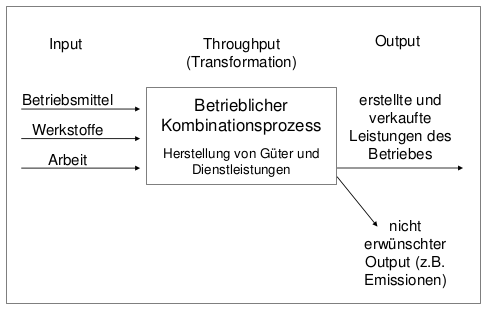
\includegraphics[width=250px]{./pictures/produktion_als_kombpr.png}
\caption{Produktion als Kombinationsprozess}
\end{figure} 

\(\rightarrow\) Ziele in dem obgigen Kombinationsprozess:
Beim Input ist die Verbesserung des Faktoreinsatzes, also eine Erhöhung der Produktivität das Ziel.
In der Transformation bzw dem Throughput ist eine Steigerung der Ausbringungsmenge bzw eine maximale Kapazitätsauslastung, sowie eine Verkürzung der Durchlauf- oder Produktionszeiten und eine Minimierung der Produktionskosten das Ziel.
Im Output wird die Steigerung des Qualitätsniveaus + der Zuverlässigkeit, sowie die Verbesserung der Arbeitsbedingungen oder des Umweltschutzes als Ziel anvisiert.

\subsubsection{Ziele \& Zielkonflikte produktionswirtschaftlicher Betätigung}
\label{sec:org137b27e}
\begin{enumerate}
\item Inhaltliche Ziele \& Zielkonflikte
\label{sec:org1b1d9d3}
Man kann inhatlich zwischen dem Werziel Produktivität, dem Humanziel Flexibilität und dem Sachziel Qualität unterscheiden. Die Ziehlbeziehungen dieser Ziele sind indifferent, komplementär und/oder konkurrierend.

\begin{figure}[htbp]
\centering
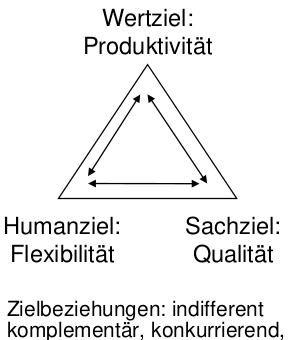
\includegraphics[width=250px]{./pictures/inhaltziele.png}
\caption{Inhaltliche Zielbeziehungen}
\end{figure} 

\item Unternehmensbeteiligte \& Interessenkonflikte
\label{sec:orgf518521}
Innerhalb des Unternehmens kann es zu diversen Konflikten \& Spannung zwischen den verschiedenen Beteiligten kommen.

Ziele/Interessen der jeweiligen Unternehmensbeteiligten:
\begin{itemize}
\item Kapitalgeber: Rentabilität des eingesetzten Kapitals
\item Mitarbeiter: ihrem Leistungsbeitrag entsprechende Anreizstrukturen (Entlohnung)
\item Lieferanten/Kunden: Absatzsicherheit, Liefersicherheit, Qualität und Liquidität
\item Öffentlichkeit: Nachhaltigkeit, Transparenz
\end{itemize}

\item Sachliche Ziele produktionswirtschaftlicher Betätigung
\label{sec:orge818be5}

\textbf{\textbf{Produktionsziele}}:
Aus dem produktionswirtschaftlichen Sachziel der Herstellung von Gütern und/oder Dienstleistungen nach Mengen-, Zeit- und Qualitätskriterien leiten sich die
produktionswirtschaftlichen Teilziele ab.
\begin{itemize}
\item Bestimmung von Anspruchsniveaus
\item Abbildung von Wirkungszusammenhängen
\end{itemize}

\textbf{\textbf{Produktionsstrategien}}:
Das Produktionssystem wird durch strategische Maßnahmen in die Lage versetzt, seine Potenziale so aufzubauen, dass sie den zukünftig auftretenden Anforderungen gerecht werden (SWOT-Analyse).

\textbf{\textbf{Produktionspolitik}}:
Die auf die Produktionsebene "heruntergebrochenen" Ziele des Unternehmens finden in der Produktionspolitik ihre Gestaltungs- und Entscheidungsmodelle
\end{enumerate}
\subsection{Ressourcenbereitstellung als nachhaltiger Wettbewerbsvorteil}
\label{sec:org7969562}
\subsubsection{Produktionssysteme(-verfahren)}
\label{sec:orge2dcdb0}
In einer gegebenen Situation wird aus allen möglichen Produkten \& Dienstleistungen ein \textbf{Produktionsprogramm} zusammengesetzt (Zielfunktion). Bei der betriebswirtschaftlichen Analyse des Produktionsprozesses sind alle Situationen \& Veränderungsmöglichkeiten zu betrachten, die auf die Zielfunktion und die Nebenbedingungen einwirken.

Das \textbf{Produktionsverfahren} bezeichnet die organisatorische \& technologische Art, in welcher ein Betrieb Produktionsfaktoren kombinieren und wie er diesen Prozess durchführt.

\subsubsection{Produktionsfunktion und Produktionsmodelle}
\label{sec:org4650393}
\begin{center}
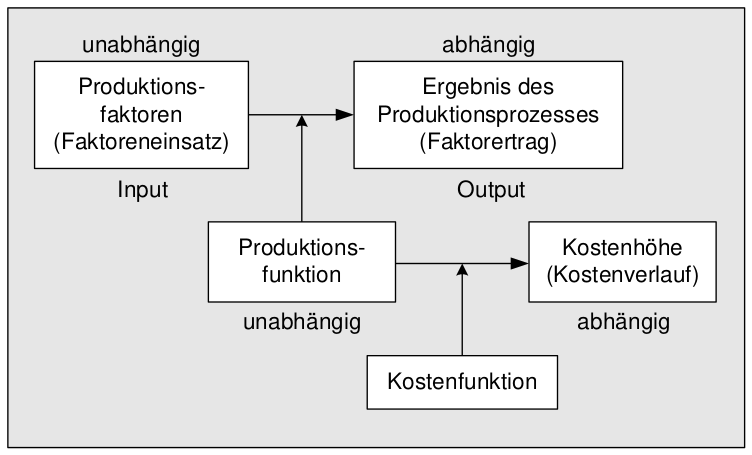
\includegraphics[width=250px]{./pictures/prodfunktion.png}
\end{center} 

Beispiel einer Produktionsfunktion: \(x=f(r_1, r_2, r_3)\)

\textbf{Kombinationsprinzip}:\\
Zur betrieblichen Leistungserstellung in einer Periode \(x\) (= Ausbringungsmenge/Output) sind alle drei Einsatzfaktoren (resources) \(r_1\) (= Verbrauch Werkstoff/Menge), \(r_2\) (= Einsaz Arbeitsstunden), \(r_3\) (= Einsatz Maschinenstunden) notwendig. Ist einer dieser Faktoren nicht vorhanden, kommt keine Leistungserstellung zustande.

\textbf{Faktorproportionsprinzip}:\\
Die Wahl der Faktorkombination \(f\) bestimmt das Verhältnis, indem die drei Faktoren miteinander kombiniert werden.

\textbf{Effizienzprinzip}:\\
Die Menge der Produktionsfaktoren, die zur Herstellung von \(x\) notwendig ist, wird bei gegebener Produktionsfunktion \(f\) genau bestimmt. Mit einem geringeren Faktorverbrauch kann \(x\) nicht hergestellt werden. Werden mehr Faktoren verbraucht liegt Verschwendung vor.

\begin{enumerate}
\item Produktionstheoretische Grundbegriffe
\label{sec:org743ed87}
\begin{itemize}
\item \textbf{Grenzrate der Faktorsubstitution} = Austauschrelation zwischen zwei Produktionsfaktoren \(r_1\) und \(r_2\) bei Konstanz der Ausbringungsmenge x
\item \textbf{Grenzproduktivität} = Veränderung der Ausbringungsmenge x in Abhängikeit von infinitisemal kleinen Änderungen der Faktoreinsatzmengen \(r_1\) bzw \(r_2\)
\item \textbf{Durchschnittsertrag} = Durchschnittlicher Ertrag des Produktionsfaktors \(r_1\) bzw \(r_2\)
\item \textbf{Produktionskoeffizient} = Anzahl der im Produktionsprozess durchschnittlich notwendigen Faktoreinsatzmengen \(r_1\) bzw \(r_2\) zur Produktion einer Einheit z
\end{itemize}

\item Kostenfunktion: Bewertung des Faktoreinsatzes
\label{sec:orgc4edbdf}
\$K = f(x)\$\\
\begin{itemize}
\item \textbf{Kosten/Gesamtkosten} = Die mit Preisen bewertete Faktoreinsatzmengen, die während einer Rechnungsperiode in Abhängikeit von dem Beschäftigungsgrad anfallen
\item \textbf{Kostenrate/Stückkosten} = Der Betrag der auf eine Leistungseinheit entfallenden Kosten (bei Angabe der Ausbringungsmenge in Stück)
\item \textbf{Grenzkosten} = Geben für jeden Beschäftigungsgrad x den Anstieg der Gesamtkostenkurve an
\item \textbf{Fixe Kosten} = Kosten der Betriebsbereitschaft, unabhängig von der tatsächlichen Leistung, zB Zinsen, Mieten, Abschreibungen
\begin{itemize}
\item Nutzkosten/Leerkosten = Abgrenzung der Kostenwirkungen der nicht beanspruchten Kapazitäten
\end{itemize}
\item \textbf{Variable Kosten} = Kosten in Abhängikeit von der tatsächlichen Leistung (proportionale, degressive, progressive Kostenverläufe)
\end{itemize}

\item Grundlegende Kritikpunkte
\label{sec:org3f058a1}
\begin{itemize}
\item mangelnde Untersuchung der Dynamik \& Unsicherheit des Produktionsgeschehens
\item ungenügende Einbeziehung der betrieblichen Organisationsstruktur
\item nicht ausreichende Berücksichtigung von Führungstätigkeiten
\item Beschränkung auf quantitative Größen
\item ungenügende Erfassung von Dienstleistungen
\item zu hohe Aggregation und zu geringe empirische Fundierung der verwendeten Größen
\end{itemize}
\end{enumerate}

\subsubsection{Produktionskonzepte und - strategien}
\label{sec:org5fe2795}
\begin{itemize}
\item Qualitätsorientierung
\item Best-practive Orientierung
\item Lernende Organisation
\item Mitarbeiter-orientierte Prozesse
\item nicht imitierbare Ressourcen wie bswp Patente, besonders einzigartige Standpunkte oder Assets sind wertvollere Ressourcen als leicht imitierbare Ressourcen wie bspw Cash oder Rohstoffe \(\rightarrow\) Generierung nicht-imitierbarer Produktionsfähigkeiten
\item Identifikation oder Entwicklung geschützter Ressourcenpositionen
\end{itemize}
\section{Finanzmanagement}
\label{sec:org44043d1}
Funktion des Finanzmanagement ist die zielgerichtete Gestaltung der betrieblichen Finanzwirtschaft:
\begin{itemize}
\item aktive Gestaltung der Kapitalzuführung und des Kapitalentzugs
\item eher passive Gestaltung der internen Finanzbewegungen
\item bezeichnet auch die mit den Managementaufgaben Finanzierung \& Finanzwirtschaft verantwortlich betrauten Mitglieder einer Organisation
\end{itemize}
\subsection{Finanzierung \& Wettbewerbsfähigkeit}
\label{sec:org24c92f4}
Ziel der Finanzwirtschaft ist die Erreichung des finanzwirtschaftlichen Gleichgewichts
\subsubsection{Zahlungsstrom, Finanzierungsmaßnahme, Kapitalveränderung}
\label{sec:orgb598bf8}
\begin{itemize}
\item \textbf{klassischer Kapitalbegriff} = Kapital ist die abstrakte Wertsumme der Bilanz; Kapital zeigt die Herkunft der Werte des Unternehmens an, unterteilt in Eigen- und Fremdkapital
\item \textbf{monetärer Kapitalbegriff} = Kapital sind im Unternehmen eingesetzte Geldmittel
\end{itemize}

Finanzwirtschaft umfasst die Kapitalbeschaffung und -verwendung der Unternehmung

\begin{enumerate}
\item Kapitalströme
\label{sec:orga499bb9}
\begin{figure}[htbp]
\centering
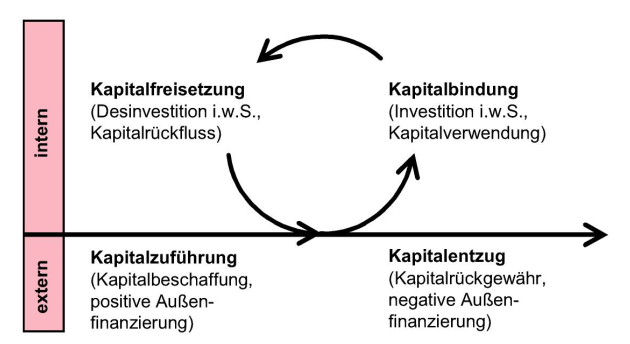
\includegraphics[width=250px]{./pictures/kapitalstroeme.png}
\caption{Kapitalveränderung als Strömungsgröße}
\end{figure} 
\begin{itemize}
\item Kapitalbindung (oder -verwendung)
\item Kapitalfreisetzung (oder -rückfluss)
\item Kapitalzuführung (oder -beschaffung)
\item Kapitalentzug (oder -abfluss)
\end{itemize}

\item Finanzielles Gleichgewicht
\label{sec:org75e022d}
\begin{figure}[htbp]
\centering
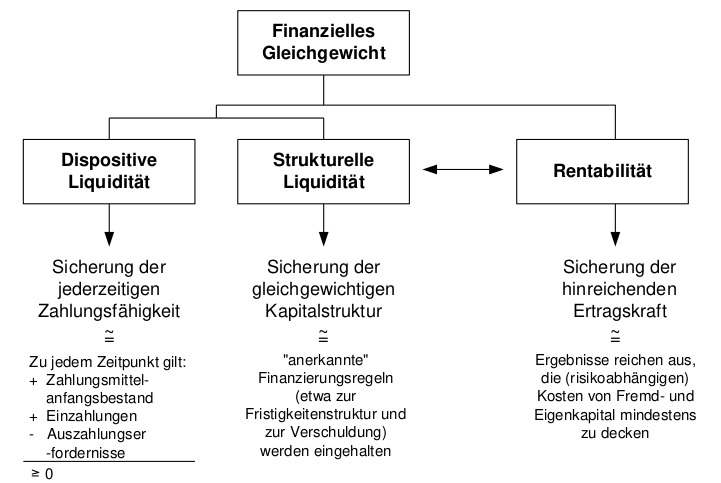
\includegraphics[width=250px]{./pictures/finanzgg.png}
\caption{Komponenten des finanziellen Gleichgewichts}
\end{figure}
\end{enumerate}
\subsubsection{Zahlungsbeziehungen, Finanzierungsform, Finanzierungsverträge}
\label{sec:org71684f6}
\begin{enumerate}
\item Zahlungsbeziehungen
\label{sec:org2e27929}
F.14 II\(_{\text{FInanzmnfgm}}\)\(_{\text{1.pdf}}\)
\item Herkunft von Finanzmitteln
\label{sec:org879cac8}
\textbf{Außenfinanzierung} \(\rightarrow\) = \textbf{Kapitalzuführung}
\begin{itemize}
\item finanzielle Mittel oder geldwertäquivalente Vermögensgegenstände werden dem Unternehmen \emph{explizit} von auf Finanzierungsmärkten (also \emph{außerhalb}) operierenden Financiers zur Verfügung gestellt
\begin{itemize}
\item Geldmarkt: Finanzmittel mit kurzer Laufzeit (zB Bank-, Kunden-, Lieferantenkredite)
\item Kapitalmarkt: Finanzmittel mit mittlerer \& längerer Laufzeit (zB Darlehen, Hypotheken, Anleihungen, Beteiligungen)
\end{itemize}
\end{itemize}

\textbf{Innenfinanzierung} \(\rightarrow\) = \textbf{Kapitalfreisetzung}
\begin{itemize}
\item finanzielle Mittel die dem Unternehmen in Form eines (positiven) Saldos zwischen Einzahlungen aus Nicht-Finanzierungsmärkten \& Auszahlungen an diese Märkte in einer Periode zugeflossen sind, werden am Verlassen des Unternehmens gehindert (\emph{innerhalb})
\begin{itemize}
\item der finanz. Überschuss wird als Cash-Flow bezeichnet und drückt die Innenfinanzierung eines Unternehmens aus
\end{itemize}
\end{itemize}
\item Finanzierungsverträge
\label{sec:org2ac5b82}
Ein Finanzierungsvertrag hält die Bedingungen fest zu denen ein Unternehmen finanzielle Mittel beschafft:
\begin{itemize}
\item Höhe \& Zeitpunkt
\item Sicherheitsgrad der Zahlungen
\end{itemize}

Es gibt 3 Formen von Finanzierungsverträgen:

\begin{enumerate}
\item Unbedingter Finanzierungsvetrag
Das Unternehmen leistet bestimmte, vertragliche fixierte Zins- und Tilgungszahlungen immer \& unter allen Umständen an den Geldgeber (zB standardisierter Kreditvertrag)

\item Bedingter Finanzierungsvertrag
Das Unternehmen leistet präzisierte Zahlungen an den Geldgeber, wenn bestimmte Bedingungen erfüllt sind (zB positiver Jahresabschluss bei Gewinnobligationen, Genussscheinen, Stamm- oder Vorzugsaktion)

\item Sicherungsvertrag
Das Unternehmen vereinbart Maßnahmen zur Besicherung der Finanzierungsmaßnahme sowie zu Informations- und Kontrollrechten des Geldgebers
\end{enumerate}
\end{enumerate}

\subsubsection{Optimale Finanzierung \& Wettbewerbsfähigkeit}
\label{sec:org65ee8f7}
Es gibt Probleme beim Erreichen des Ziels der optimalen Finanzierung. Die Konsequenzen von Investitionsprogrammen \& Finanzierungsverträgen sind für Eigentümer \& Gläubiger nicht vollständig bekannt, außerdem sind ihre Erwartungen unterschiedlich. Finanzierung kann außerdem Hinblick auf verschiedene andere Ziele/Faktoren betrachtet werden:

\begin{enumerate}
\item Finanzierung \& Liquidität
Sicherung der Zahlungsfähigkeit innerhalb eines gegebenen Planungszeitraums

\item Finanzierung \& Rentabilität
Konsistente Aussagen zum erwarteten Erfolg investierter Mittel / im Vergleich von Planungszeitraum / ggü dem Kapitalmarkt

\item Finanzierung \& Risiko
Prognose des Eintritts des erwarteten Erfolgs investiertet Mittel (Eintrittswahrscheinlichkeit) / Finanzierungsverträge zur Risikoteilung bei Eigen- und Fremdfinanzierung
\end{enumerate}

II\(_{\text{Finanzmanagement}}\)\(_{\text{2.pdf}}\) -> F.6 Zusammenfassung

\subsection{Bereitstellung finanzieller Ressourcen}
\label{sec:org086b84a}
\subsubsection{Formen der Finanzierung}
\label{sec:org469b664}
\begin{center}
\begin{tabular}{lll}
Herkunft der Finanzmittel/Rechtsstellung des Kapitalgebers & Eigenfinanzierung (Eigentümer) & Fremdfinanzierung (Gläubiger)\\
\hline
Außenfinanzierung & Beteiligungsfinanzierung & Kreditfinanzierung\\
Innenfinanzierung & Selbstfinanzierung (insbs. aus Gewinnen) & Sonstige (insbs. Rückstellungen)\\
\end{tabular}
\end{center}

\textbf{Beteiligungsfinanzierung} = Finanzierung durch (bisherige oder neue) Eigentümer
\begin{itemize}
\item Eigenkapital (von außen zugeführt oder entsprechende Sacheinlagen der Eigentümer)
\item Beteiligungskapital
\begin{itemize}
\item Beschaffung von Eigenkapital durch Aufnahme neuer Teilhaber (Gesellschafter) bei nicht emissionsfähigen Unternehmen
\item Beschaffung von Eigenkapital bei emissionfähigen Unternehmen (Stammaktie/Vorzugsaktie/Genussschein)
\end{itemize}
\end{itemize}

\textbf{Kreditfinanzierung} = Finanzierung durch externe Kapitalgeber (Gläubiger)
\begin{itemize}
\item Formen der langfristigen Kreditfinanzierung über den Kapitalmarkt
\begin{itemize}
\item Schuldverschreibung, Industrieanleihe
\item Schuldscheindarlehen, Investitionsdarlehen
\end{itemize}
\item Formen der kurzfristigen Kreditfinanzierung über den Geldmarkt
\begin{itemize}
\item Bank-/Handels-/Lieferantenkredite
\end{itemize}
\item Sonderformen
\begin{itemize}
\item Factoring, Leasing
\end{itemize}
\end{itemize}

\begin{center}
\begin{tabular}{lll}
Vergleichskriterium & Beteiligungsfinanzierung & Kreditfinanzierung\\
\hline
Anspruchsgrundlage & Quotenanteil & Nominalanspruch\\
Erfolgsansrpuch & erfolgsabhängig/variabel & erfolgsunabhängig/kontraktbestimmt\\
Befristung & Nein & Ja\\
Haftung & Ja zumindest begrenzt & Nein\\
Leitung & Ja zumindest begrenzt & Nein\\
\end{tabular}
\end{center}

\begin{enumerate}
\item Wahl der optimalen Finanzierung
\label{sec:org399b92d}
\textbf{Finanzierung \& Risiko/Chance}
\begin{itemize}
\item Financiers werden - unter sonst gleichen Bedingungen - eine Finanzierung umso besser einschätzen, je sicherer die in Aussicht gestellten Renditen sind
\begin{itemize}
\item Risiko/Chance kann gleichgesetzt werden mit der Möglichkeit des Eintreten eines ggü dem Erwartungswert nachteiligen/vorteilhaften finanz. Ereignisses/Ergebnisses
\item Risiko/Chance liegt dann vor, wennn eine eingetretene Nettoeinzahlung (finanzielles Ergebnis) unterhalb/oberhalb des eingesetzten Kapitals liegt
\end{itemize}
\end{itemize}

\textbf{Liquidität (finanz. Gleichgewicht)}
\begin{itemize}
\item ein Unternehmen ist liquide (zahlungsfähig), wenn es in der Lage ist, seinen Zahlungsverpflichtungen innerhalb eines gegebenen Planungszeitraums jederzeit vertragskonform nachzukommen
\begin{itemize}
\item Zahlungsfähigkeit = Zahlungsvermögen > Zahlungsverpflichtungen
\end{itemize}
\item \emph{Risiko der Liquidität}: Aufrechterhaltung der Liquidität ist eine notwendige Voraussetzung für den Fortbestand eines Unternehmens. Aktuelle oder drohende Zahlungsunfähigkeit oder eine Überschuldung sind Gründe für eine Insolvenz
\end{itemize}

\textbf{Rentabilität}
\begin{itemize}
\item Rentabilität spiegelt das Ergebnis unternehmerischer Tätigkeit wieder, in dem der finanzwirtsch. Erfolg in Relation zum eingesetzten Kapital gesetzt wird 
\begin{itemize}
\item Eigenkapital, Gesamtkapital, Umsatz
\end{itemize}
\item \emph{Risiko der Rentabilität}: zur zukunftsgerichteten Begründung von Entscheidung ist mit Erwartungswerten zu rechnen, die an Bedeutung verlieren, je größer die Unsicherheit ist
\end{itemize}
\end{enumerate}

\subsection{Finanzierungsplanung}
\label{sec:orgb89b2b0}
\begin{enumerate}
\item Begriff \& Arten der Liquidität
\label{sec:orga9aa41c}
Ein Unternhemen ist \emph{liquide} (zahlungsfähig), wenn es in der Lage ist, seinen Zahlungsverpflichtungen innerhalbs eines gegebenen Planungszeitraums jederzeit vertragskonform nachzukommen. Die Aufrechterhaltung der Liquidität ist eine notwendikge Voraussetzung für den Fortbestand eines Unternehmens. Aktuelle oder drohende Zahlungsunfähigkeit oder eine Überschuldung sind Gründe für eine Insolvenz.

Arten der Liquidität:
\begin{itemize}
\item güterwirtschaftliche Liquidät
\item verliehende Liquidität
\item zukünftige Liquidität
\item antizipierte Liquidität
\end{itemize}

Messung von Liquidität:
\begin{itemize}
\item Beurteilung anhand der Liquiditätsgrade \& der Struktur von Kapitalbindung und -bereitstellung (horizontale Kapitalstruktur = Vergleich von Vermögen und Kapitalstruktur), sowie anhand des Verschuldungsgrads (vertikale Kapitalstruktur = Vergleich von Eigen- und Fremdkapital)
\item Beurteilung auf der Basis von Finanzplänen
\end{itemize}

II\(_{\text{Finanzmanagement}}\)\(_{\text{2.pdf}}\) F.22 Zusammenfassung
\end{enumerate}
\section{Personalmanagement}
\label{sec:orgbe6ce8a}
\subsection{Personal \& Wettbewerbsfähigkeit}
\label{sec:orge4ef43a}
Das Ausgangsproblem dreht sich um die optimale Ergiebigkeit menschlicher Arbeitsleistung (Gutenberg).

Kategorien/Ebenen personalwirtschaftlichen Handelns:
\begin{itemize}
\item Zielebene = Verfügbarkeit \& Wirksamkeit von Personal
\item Instrumentenebene = Selektion personalwirtschaftlicher Maßnahmen (Instrumente/Ergebnisse) und ihre Wirkungen (intendiert / nicht intendiert)
\item Erfolgsebene = Management der Humanressourcen und Unternehmenserfolg
\end{itemize}

\subsubsection{Personalwirtschaftliches Handeln}
\label{sec:org2172a29}
Geht man davon aus, dass ein bestimmter personalwirtschaftlicher Zweck prinzipiell durch verschiedene Handlungen erreicht werden kann, dass außerdem eine bestimmte Handlung prinzipiell verschiedenen personalwirtschaftlichen Zwecken dienen kann und dass schließlich Handlungen auch 'nicht-bezweckte'(nicht-intendierte) Wirkungen hervorrufen können, so werden \emph{Wahlprobleme} sichtbar, die sich mit Hilfe von elementaren \emph{Kategorien} charakterisieren lassen.

Personalwirtschaftl. Probleme entstehen, wenn Unternehmer andere Personen zur Deckung des Arbeitskräftebedarfs in einer Weise in Dienst stellen dass diese bestimmte Dispositionsbefugnisse über ihre Arbeitskraft gegen eine festgelegte Vergütung direkt oder indirekt auf den Unternehmer übertragen.

Prolemkategorien:
\begin{itemize}
\item Herstellung \& Sicherung der Verfügbarkeit \emph{über} Personal (\textbf{Disponibilität})
\begin{itemize}
\item menschliche Arbeitskraft ist ein knappes "Gut"
\item menschliche Arbeitskraft wird in versch Qualität nachgefragt \& angeboten
\item der Bedarf des Betriebes an Personal verändert sich quantitativ und/oder strukturell
\item eine zu einem bestimmten Zeitpunkt gegebene Ausstattung eines Betriebes mit Personal unterliegt im Zeitablauf quantitativen und/oder strukturellen Veränderungen, die nicht durch betriebliche Dispositionen induziert werden
\end{itemize}
\item Herstellung \& Sicherung der Verfügbarkeit \emph{des} Personal (\textbf{Funktionalität})
\begin{itemize}
\item Ansprüche an das Verhalten des Personals sind je nach Situation bzgl ihres konkreten Inhalts und ihres relativen Gewichts unterschiedlich
\item Personal wird idR aufgrund von Selbstdarstellung, Fremdeinschätzung \& Verhaltensstichproben ausgewählt, deren Aussageberich beschränkt und deren Aussagekraft häufig gering sind
\item die Annahme, das sich die Arbeitskräfte mit den Verhaltensansprüchen der Organisation identifizieren, trifft im Regelfall weder für die Verhaltensansprüche noch für alle Angehörigen eines Betriebens in gleicher Weise zu
\item die Erfüllung von Verhaltensansprüchen muss den Mitarbeitern möglich sein
\end{itemize}
\end{itemize}

\subsubsection{Instrumentenebende personalwirtschaftlichen Handelns}
\label{sec:org92ff445}
\begin{figure}[htbp]
\centering
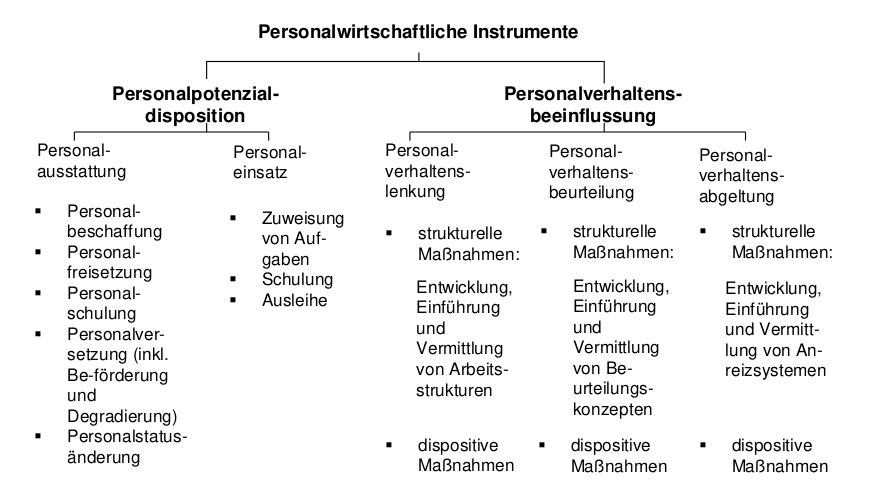
\includegraphics[width=250px]{./pictures/persinstr.png}
\caption{Instrumentenebene personalwirtschaftlichen Handelns}
\end{figure} 

\subsubsection{Zielebene personalwirtschaftlichen Handelns}
\label{sec:org49059f4}
\begin{itemize}
\item Individuelle Schutzreche
\begin{itemize}
\item Schutz des Arbeitsverhältnisses (zB Kündigungsschutz)
\item Schutz der Gesundheit (zB Emissionschutz, Arbeitsschutz)
\item besondere Schutzrechte (zB für gefährdete Mitarbeitergruppen)
\end{itemize}
\item Arbeitsrechtliche Mitbestimmung
\begin{itemize}
\item Beteiligung bei sozialen \& personellen Entscheidungen
\item Informations-, Beratungs-, Mitwirkungs- und Mitbestimmungsrechte
\item Interessenvertretung durch Betriebsrat, Jugendvertretung, Wirtschaftsausschuss oä
\end{itemize}
\item Unternehmerische Mitbestimmung
\begin{itemize}
\item Mitwirkungsrechte bei unternehmerischen Entscheidungen
\end{itemize}
\end{itemize}

\subsubsection{Erfolgsebene personalwirtschaftlichen Handelns}
\label{sec:org4c4c0e0}
\begin{figure}[htbp]
\centering
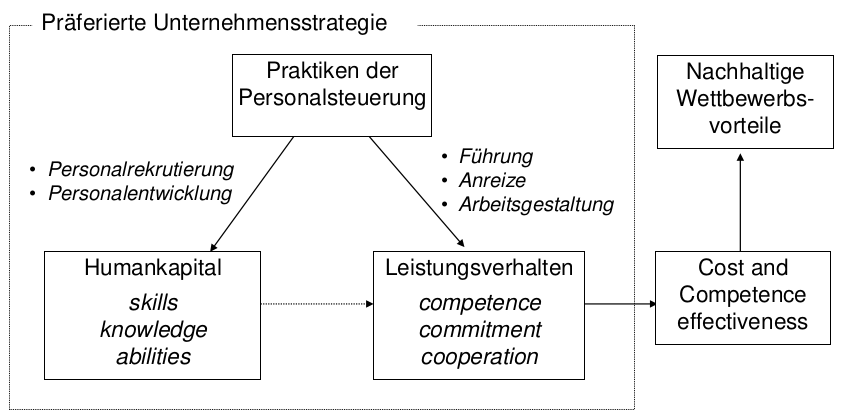
\includegraphics[width=250px]{./pictures/perserfolg.png}
\caption{Management der Humanressourcen \& Unternehmenserfolg}
\end{figure} 
\subsubsection{Elementarkategorien personalwirtsch Handelns (Zusammenfassung)}
\label{sec:org0c278bc}
\begin{figure}[htbp]
\centering
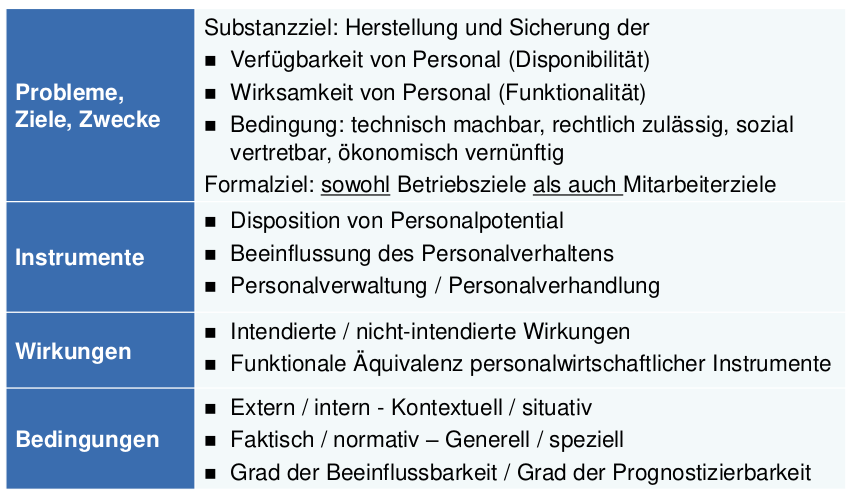
\includegraphics[width=250px]{./pictures/perskateg.png}
\caption{Instrumentenebene personalwirtschaftlichen Handelns}
\end{figure} 

\subsection{Disposition des Personalpotentials}
\label{sec:org1bb50b3}
\subsubsection{Personalbedarf}
\label{sec:org6c99c0e}
Der \emph{Personalbedarf} einer Organisation umfasst - nach geforderten Qualifikationsstrukturen - gruppiert die Gesamtheit, die zur Wahrnehmung aller dispositiven \& exekutiven Aufgaben in allen Bereichen und auf allen Ebenen einer Organisation benötigt werden.

Primärdeterminanten:
\begin{itemize}
\item periodenbezogenes Leistungsprogramm eines Betriebes
\item Arbeitszeitbedarf pro Leistungseinheit (Arbeitskoeffizient) bzw pro zu bedienender Bestandseinheit (Besetzungskoeffizient)
\item verfügbare Arbeitszeit der Arbeitskraft pro Periode
\end{itemize}

Sekundärdeterminanten:
\begin{itemize}
\item Angebots-/Nachfrageverhältnis, Technologie (zB Automatisierungsgrad), Grad der Arbeitsteilung
\item Anforderungsprofile/Stellenbeschreibungen
\end{itemize}

Verfügbarkeit des Personals \(\rightarrow\) Dispositionsabhängigkeit der Bestimmung \& Deckung des Personalbedarfs
\subsubsection{Personalrekrutierung und -auswahl}
\label{sec:org36f9d42}
Anwerbung
\begin{itemize}
\item Zweck = Herstellung von Kontakten zu potentiellen Bewerbern, Personalmarketing (Arbeitgeberimage)
\item Funktionen = Information, Motivation, Vorselektion
\item Methoden = passiv, aktiv (zB Stellenanzerigen, elektr. Jobbörsen)
\end{itemize}

Auswahl
\begin{itemize}
\item Zweck = Identifikation der Eignung von Bewerbern für eine zu besetzende Stelle/Position, Screening-Strategie
\item Phasen = Vorauswahl, Auswahl
\item Methoden = Eignungstest, Assessment Center, Auswahlgespräch
\end{itemize}

Einstellung
\begin{itemize}
\item Zweck = Vereinbarungen zum Arbeitsverhältnis und zur Arbeitsleistung
\item Inhalt = Kompetenzabgrenzung, Arbeitsbedingungen, berufliche Entwicklungsperspektiven
\item impliziter Vertrag =  Vereinbarung von Rechten \& Pflichten auf der Basis stillschweigender Übereinkünfte
\end{itemize}

Eingliederung
\begin{itemize}
\item Zweck = Einführung des Mitarbeiters in das Arbeits-/Aufgabenfeld
\item Inhalt = bereichsübergreifende, fachliche, soziale Eingliederung
\end{itemize}

Berufsbozgenes Integritätsprofil als Profil/Einschätzung der Eignung. Baumquerschnittdiagramm mit verschiedenen Charaktereigenschaften wie Gelassenheit, Vertrauen, Zuverlässigkeit, Verzicht auf Rechtfertigung etc.

\textbf{Einstellungsinterviews}\\
unstrukturiertes Interview:
\begin{itemize}
\item Annahmen über Menschenkenntnis
\item Unterstützung von Stereotypen
\item Annahmen über ideale Persönlichkeit
\item hohe Wirkung von non-verbalem Verhalten
\end{itemize}

strukturiertes Interview:
\begin{itemize}
\item anforderungsbezogene Gestaltung
\item Interviewverlauf und Fragenabfolge sind strukturiert
\item Verwendung validierter/bewährter Merkmale
\item Information \& Entscheidung sind getrennt (Beratungszeit)
\item mehrere unabhängige \& kompetente Beurteiler sind beteiligt
\end{itemize}


\begin{figure}[htbp]
\centering
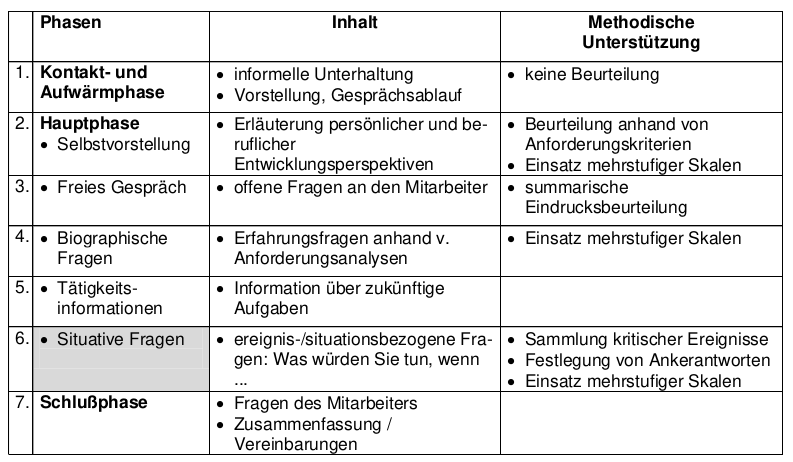
\includegraphics[width=250px]{./pictures/persint.png}
\caption{Multimodales Interview}
\end{figure} 
\subsubsection{Einsatz \& Disposition des Personals}
\label{sec:orge0b1872}
Einsatz von Personal
\begin{itemize}
\item Zweck =  Übertragung von Aufgaben oder Stellen an die vorhandenen/verfügbaren Arbeitskräfte
\item Methode = Zuordnung von Anforderungsprofilen und Fähigkeitsprofilen auf der Basis von Mindestwerten (Cut-Off Methode) oder (gewichteten) Ähnlichkeiten (Profilvergleichsmethode)
\end{itemize}

Segmentierung des Personals
\begin{itemize}
\item Differenzierung der Verfügbarkeit des Personals nach spezifischen Beschäftigungs-, Arbeits- und Entgeltbedingungen
\item Stammbelegschaft = internes Arbeitsmarktsegment
\item Randbelegschaft = externes Arbeitsmarktsegment (Manövriermasse für quantitative Anpassungen des Personalbestands)
\end{itemize}

Personalplanung als Disposition \(\rightarrow\) die Aufgabe der Personalplanung ist es, den Personalbedarf, den Personaleinsatz und die Personalaustattung - unter Beachtung der für den Personalsektor geltenden Restriktionen - optimal im Sinne der betrieblichen Ziele aufeinander abzustimmen
\subsubsection{Personalentwicklung}
\label{sec:orga3653f7}
\begin{figure}[htbp]
\centering
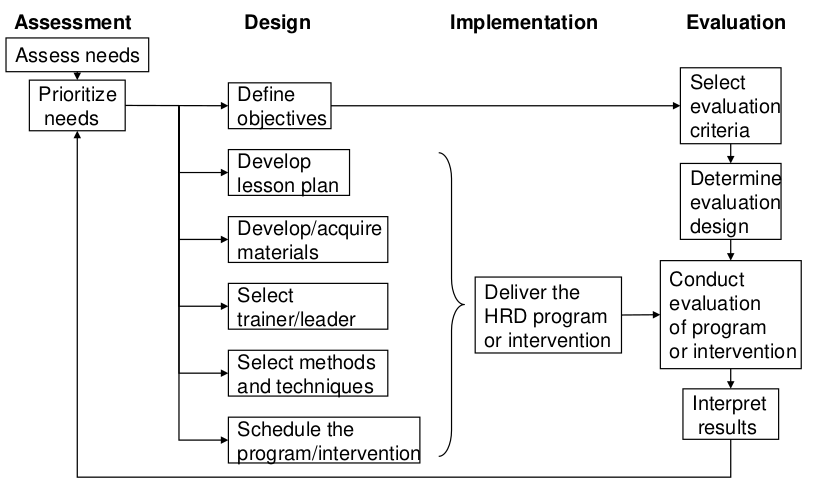
\includegraphics[width=250px]{./pictures/persgruent.png}
\caption{Grundmodell der Personalentwicklung}
\end{figure} 

Beeinflussung des Personalverhaltens nicht klausurrelevant!

\textbf{Ansprüche als Kriterium der Verhaltensbeeinflussung}:

Beeinflussung des Personalverhaltens
\begin{itemize}
\item Zweck = Durchsetzung von Ansprüchen der Organisation an das Personalverhalten (Verhaltenserwartung)
\item Inhalt = Aufforderung, sich in einer bestimmten Art \& Weise zu Verhalten (Anspruchskonformität des Verhaltens)
\end{itemize}

Inhaltsklassen organisationaler Ansprüche
\begin{itemize}
\item Funktional = Verhaltenserwartungen, die sich auf die Arbeitsaufgaben und die Arbeitsergebniise beziehen (\(\rightarrow\) Qualitätsansprüche, Gestaltungsansprüche)
\item Extrafunktional = Verhaltenserwartungen, die sich insbes auf das Sozialverhalten beziehen (\(\rightarrow\) Höflichkeit, Ehrlichkeit, Pünktlichkeit)
\item Situationsabhängigkeit von Verhaltenserwartungen
\end{itemize}

Maßnahmen zur Verhaltensbeeinflussung
\begin{itemize}
\item Verhaltenslenkung
\item Verhaltensbeurteilung
\item Verhaltensabgeltung
\end{itemize}


\textbf{Strukturelle Maßnahmen zur Beeinflussung des Personalverhaltens}
\begin{itemize}
\item strukturelle Maßnahmen = Arbeitsstruktur, Beurteilung, Anreize
\item Entlohnung als Anreiz
\end{itemize}
\begin{figure}[htbp]
\centering
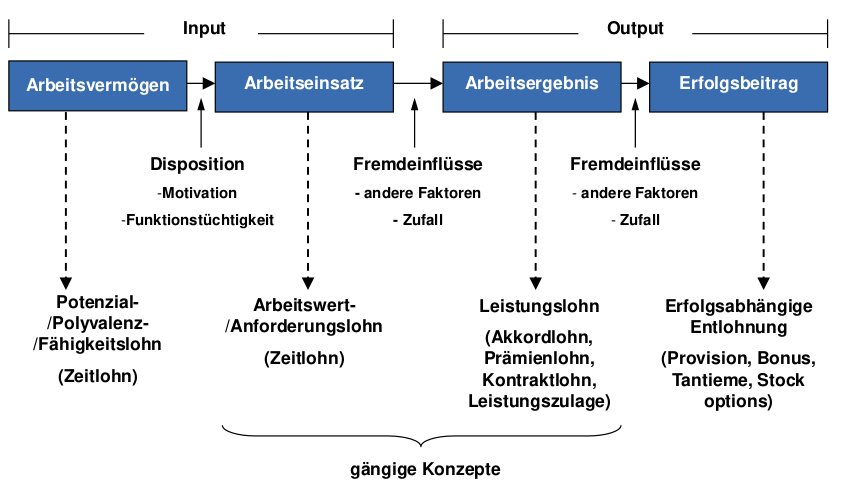
\includegraphics[width=250px]{./pictures/persentl.png}
\caption{Bemessungsgrundlagen \& Formen der Entlohnung}
\end{figure} 



\textbf{Dispositive Maßnahmen zur Beeinflussung des Personalverhaltens}
\begin{itemize}
\item dispositive Maßnahmen = Beeinflussung durch situationsabhängies Führungsverhalten
\item Führungskonzept, Situation und Führungserfolg
\begin{itemize}
\item Kontingenzmodell der Führung nach Fiedler
\item Situative Führungstheorie nach Hersey/Blanchard
\end{itemize}
\end{itemize}

III\(_{\text{Personalmanagement}}\)\(_{\text{3.pdf}}\) F.13 Zsmfassung
\section{Innovationsmanagement}
\label{sec:org7f0f914}
\subsection{Technologischer Wandel \& Wettbewerbsfähigkeit}
\label{sec:orgc92a881}
\begin{itemize}
\item Ausgangsproblem = Optimale Ergiebigkeit der Betriebsmittel
\item Technischer Fortschritt \& Innovationsmanagement
\begin{itemize}
\item Grundkategorien: Forschung, Entwicklung, Innovationsmanagement
\item Aufgaben der Forschung, Entwicklung \& Konstruktion
\item Aufgaben \& Ziele des Innovationsmanagements
\end{itemize}
\item Innovation \& Wettbewerbsfähigkeit
\begin{itemize}
\item Wettbewerb um F+E-Leistungen
\item Erfolgsfaktoren von Innovationen
\end{itemize}
\end{itemize}

\subsubsection{Optimale Ergiebigkeit der Betriebsmittel}
\label{sec:org6acb09c}
Betriebsmittel sind die gesamte technische Apparatur, deren sich ein Unternehmen bedient, um Sachgüter herzustellen oder Dienstleistungen bereitzustellen. Hinsichtlich der \emph{technischen Basis} kann man das Leistungspotential der Betriebsmittel abhängig vom \emph{Grad der Modernität}, \emph{Grad der Abnutzung} und dem \emph{Zustand an Betriebsfähigkeit} feststellen.

Technische Eignung 
\begin{itemize}
\item = das Verhältnis zwischen der vom Betriebsmittel verlangten \& der mit ihm tatsächlich erzielbaren Leistung
\item \emph{Wirkungsgrad}: Maximalkapazität, Minimalkapazität, Optimalkapazität, Kapazitätsreserven
\item \emph{Auslastungsgrad}: Ausschöpfung des qualitativen Leistungspotentials
\item \emph{Flexibilitätsgrad}: Universalmaschinen, Sondermaschinen, betriebstechnische Elastizität/Umstellungsaufwand
\end{itemize}

\subsubsection{Forschung, Entwicklung und Innovation}
\label{sec:org193ee77}
\emph{Technischer Fortschritt} bezeichnet die Veränderung und zugleich technische Verbesserung von Produktionsfaktoren, Produktionsprozessen und Produkten \(\rightarrow\) Aufrechterhaltung der technologischen Wettbewerbsfähigkeit.

\emph{Forschung} und \emph{Entwicklung} beschreibt die systematische Gewinnung neuer wissenschaftlicher und technischer Erkenntnisse, mit deren Hilfe die unternehmerischen Ziele besser als bisher erreicht werden.
\begin{itemize}
\item Grundlagenforschung, angewandte Forschung
\item Forschung, Entwicklung + Konstruktion
\end{itemize}

Eine \emph{Innovation} bezeichnet eine technische Verbesserung von Produktionsfaktoren, Produktionsprozessen und Produkten, die einen Neuheitswert besitzt und für deren Angebot eine Nachfrage besteht.

\subsubsection{Aufgaben in der Forschung und Entwicklung}
\label{sec:org405069e}
\begin{figure}[htbp]
\centering
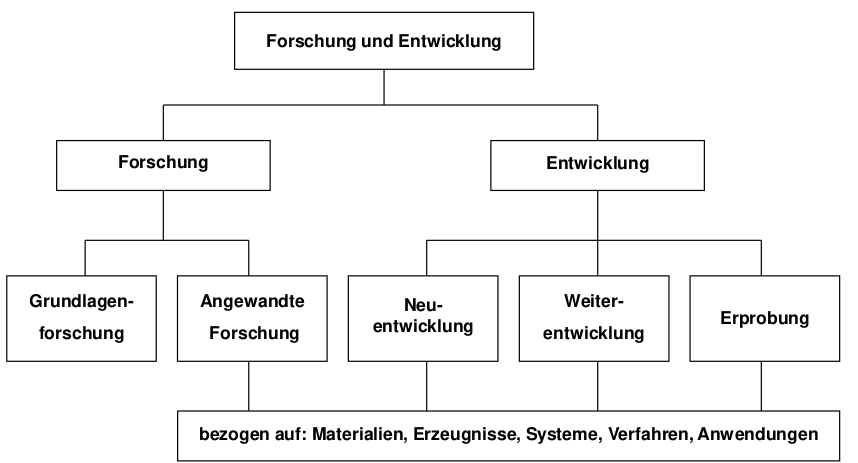
\includegraphics[width=250px]{./pictures/inaufg.png}
\caption{Aufgabenfelder}
\end{figure} 

\subsubsection{Dimensionen der Innovation}
\label{sec:org802233a}
Wenn in der Betriebswirtschaftslehre von \emph{Innovationen} gesprochen wird, sind allgemein Veränderungen gemeint, die einen Neuheitswert (eine Neuartigkeit) besitzen. Mit Innovationen wird sowohl der Prozess als auch sein Ergebnis bezeichnet, wofür die Eigenschaft der Neuartigkeit zutrifft.
\begin{itemize}
\item qualitativ neuartige Produkte oder Verfahren, die sich ggü einem Vergleichszustand "merklich" unterscheiden
\begin{itemize}
\item Produktinnovationen, Produktionsverfahreninnovationen, Anwendungsinnovationen
\item Marktinnovationen (Erschließung neuer Märkte)
\item sonstige Innovatioen (Qualitätsverbesserung, sowie schnellere Bearbeitung oä)
\end{itemize}
\end{itemize}

Neuheitsgrad
\begin{itemize}
\item Ausprägung der Neuheit zu einem bestimmten Zeitpunkt
\item Invention (Erfindung), Imitation, Variation/Modifikation
\end{itemize}

Neuheitsumfang
\begin{itemize}
\item subjektiv empfundener Verlust (Nutzenschwund) der Neuheit im Zeitverlauf
\item Veränderung mit dem Lebenszyklus einer Neuheit
\item Schwund, Alterung, Verfall
\end{itemize}

Neuheitswert
\begin{itemize}
\item Messung der Vorteilhaftigkeit (Bewertung) von Innovationen im Wettbewerb
\end{itemize}

Dimensionen von Innovationen
\begin{itemize}
\item Inhaltlich: Was ist neu?
\begin{itemize}
\item Produkt, Prozess, System
\item Kontinuität, Diskontinuität
\end{itemize}
\item Intensität: Wie neu?
\begin{itemize}
\item Neu der Tatsache nach oder Neu dem Grade nach
\item Typologie von Innovationen, Multi-Dimensionalität
\end{itemize}
\item Subjektivität: Neu für wen?
\item Prozessual: Wo beginn, wo endet die Neuerung?
\begin{itemize}
\item Invention, Innovation, Imitation, Variation, Routine
\item Phasen zur Innovation
\end{itemize}
\item Normativ: Ist neu gleich erfolgreich?
\end{itemize}

\subsubsection{Aufgaben \& Ziele des Innovationsmanagements}
\label{sec:org2b5c5f9}
Merkmale von Innovationen
\begin{itemize}
\item systematisierte Suchprozesse nach neuen Ideen
\item schwache Strukturiertheit der  Innovationsprozesse
\item "reifende Prozesse"
\item innerbetriebliche, zwischenbetriebliche, behördliche \& protestbedingte Widerstände
\end{itemize}

Planungsaufgaben
\begin{itemize}
\item Motivation zu Innovationen
\item Zielvorgaben für Innovationen
\item Definition des Innovationsproblems
\item Suche nach innovativen Alternativen
\item Bewertung \& Auswahl der Innovationsprozesse (-projekte) und Formulierung eines Innovationsprogramms-/-budgets
\end{itemize}

Steuerungsaufaben
\begin{itemize}
\item Durchsetzung der Innovationsprozesse/Überwindung von Widerständen
\item Kontrolle der Innovationsprozesse
\item Sicherung der Innovationsprozesse und -ergebnisse
\end{itemize}

Weitere Aufgaben
\begin{itemize}
\item organisatorische Gliederung des Innovationsbereichs
\item personalpol. Aufgaben der Innovationsprojekte
\item Flexibilität der Innovationsprozesse
\end{itemize}

\subsubsection{Innovation und Wettbewerbsfähigkeit}
\label{sec:org6dae8bf}
\begin{figure}[htbp]
\centering
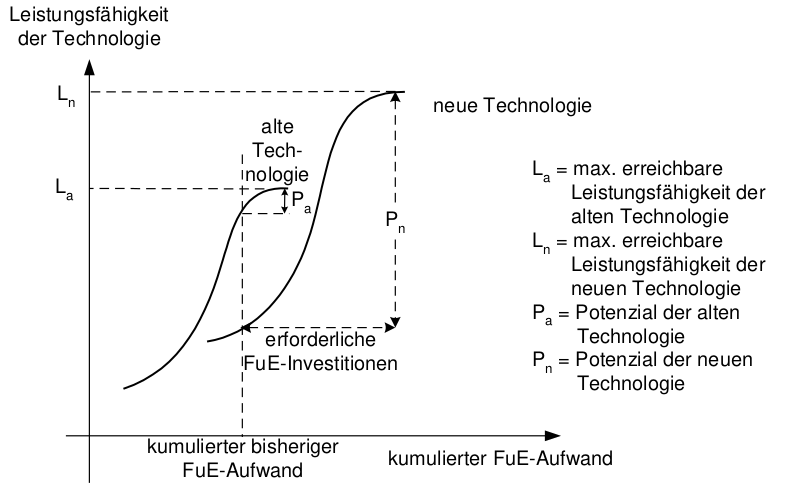
\includegraphics[width=250px]{./pictures/inskurv.png}
\caption{S-Kurven Konzept zur Technologieentwicklung}
\end{figure} 

\begin{figure}[htbp]
\centering
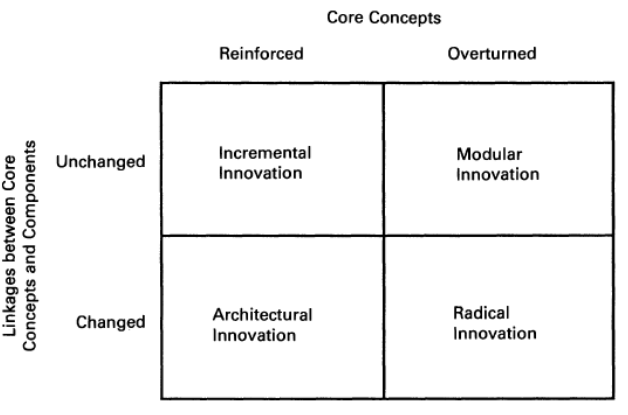
\includegraphics[width=250px]{./pictures/insfram.png}
\caption{A framework for defining innovation}
\end{figure} 

\begin{enumerate}
\item Aufgabenfelder strategischer F+E Planung
\label{sec:org315f189}
Forschungs- und Entwicklungsprogramm
\begin{itemize}
\item Schwerpunktsetzung durch Technologiestrategie
\begin{itemize}
\item Produkt- und Prozessforschung
\item Technologien
\end{itemize}
\item Allokation des F+E-Aufwands
\end{itemize}

Eigen- oder Fremdforschung
\begin{itemize}
\item Eigenforschung zur Sicherung von Wettbewerbsvorsprüngen
\item Fremdforschung als 
\begin{itemize}
\item Auftragsforschung
\item Innovationskooperation
\item Gemeinschaftsforschung
\end{itemize}
\item Übernahme externer F+E Erkenntnisse
\begin{itemize}
\item Kauf/Lizenznahme
\item Kauf innovativer Unternehmen
\end{itemize}
\end{itemize}

\item Erfolgsfaktoren von Innovation
\label{sec:org0fd0fe7}
\begin{figure}[htbp]
\centering
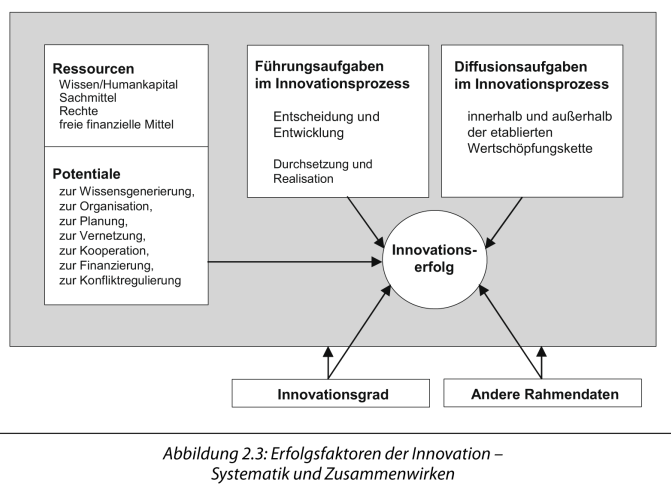
\includegraphics[width=250px]{./pictures/inerf.png}
\caption{Erfolgsfaktoren - Systematik \& Zusammenwirken}
\end{figure}
\end{enumerate}
\subsection{Strategische Forschungs- und Entwicklungsplanung}
\label{sec:orgfbe4a9b}
\subsubsection{Phasenschema des Innovationsmanagements}
\label{sec:org51ea9e5}
\begin{enumerate}
\item Planungsaufgaben der F+E
\label{sec:org18efd97}
Planungsaufgaben der Forschung \& Entwicklung sind:
\begin{itemize}
\item Zielbildung
\begin{itemize}
\item unter Zielbildung ist das Feststellen \& Festlegen eines präzisen, strukturierten \& realisierbaren Systems von Verhaltensnormen zu verstehen
\end{itemize}
\item Problemlücke
\begin{itemize}
\item als Problemlücke lässt sich die Abweichung der erwarteten Lage (Lageprognose) zum Soll-Zustand festlegen, die durch zielführende Maßnahmen der Entscheidungsträger geschlossen werden soll
\end{itemize}
\item Alternativensuche
\begin{itemize}
\item unter Alternativensuche ist das systematische Aufspüren, Formulieren und Analysieren von unabhängigen Vorgehensweisen zur Zielerreichung zu verstehen
\end{itemize}
\item Prognosen
\begin{itemize}
\item Prognosen sind Wahrscheinlichkeitsaussagen über das Auftreten von Ereignissen (Wirkungen, Daten) in der Zukunft, die auf Beobachtungen \& theoret. Aussagen beruhen
\end{itemize}
\item Bewertung
\begin{itemize}
\item unter Bewertung ist die Zuordnung einer Zielwirkung zu einer Alternative zu verstehen
\end{itemize}
\end{itemize}


Interdependenz von Zielbildungs- und Problemlösungsprozess
\begin{itemize}
\item \emph{Spezifität}: für Innovationen müssen spezifische Ziele formuliert werden, die Übernahme von Entscheidungen us anderen Zusammenhängen ist nicht möglich
\item \emph{Prozess}: eine Zielbildung ist kein zeitlich abgeschlossener Normsetzungsakt, sondern ein zeitverbrauchender, kognitiver \& konfliktregulierender Prozess (\emph{Reifungsprozess})
\item \emph{Parallelität}: Zielbildungsprozess \& Problemlösungsprozess verlaufen in unterschiedlichen Formen weitgehend parallel
\item \emph{Interdependenz}: Zielbildungsprozess \& Problemlösungsprozess sind wechselbezüglich verknüpft
\end{itemize}

\begin{figure}[htbp]
\centering
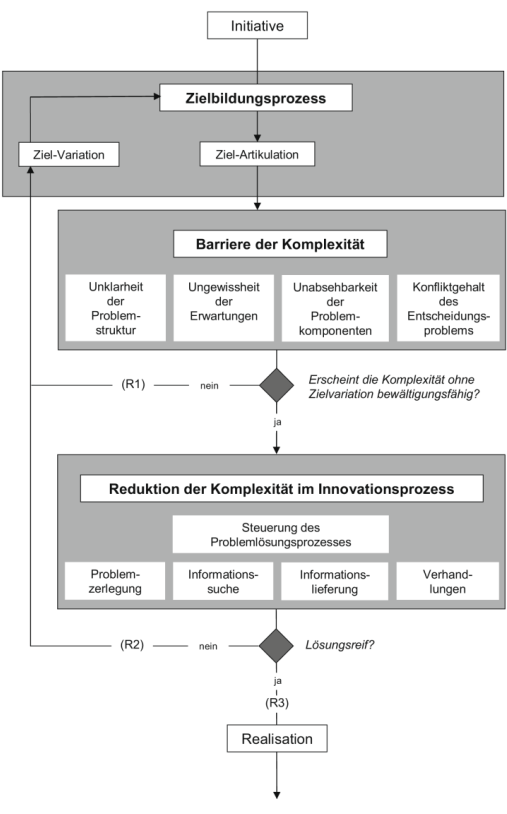
\includegraphics[width=250px]{./pictures/inziel.png}
\caption{Zielbildung im Innovationsprozess}
\end{figure} 

\item Bewertungsaufgaben der F+E
\label{sec:orgfdbd42f}
Zielbildung
\begin{itemize}
\item unter Zielbildung ist das Feststellen \& Festlegen eines präzisen, strukturierten \& realisierbaren Systems von Verhaltensnormen zu verstehen
\end{itemize}

Bewertung
\begin{itemize}
\item Aufgaben der Bewertung:
\begin{itemize}
\item Festlegung der Bewertungskriterien \& der Kriteriengewichte
\item Ermittlung der Kriterienwerte
\item Ermittlung des Gesamtwertes der Alternative
\item Wahl der Erfolg versprechenden Forschungs- und Entwicklungsalternative
\end{itemize}
\item Aufgabe der Kontrolle
\begin{itemize}
\item Ermittlung \& Analyse von Abweichung zwischen Plangrößen (Prognose- und Vorgabegrößen) und Vergleichgrößen
\end{itemize}
\end{itemize}

\item Steuerungsaufaben der F+E
\label{sec:org418a9ab}
Steuerung
\begin{itemize}
\item als Steuerung werdne geordnete informationsverarbeitende \& zielführende Eingriffe (Anpassungsmaßnahmen) in den Realisationsprozess von Forschung \& Entwicklung definiert
\end{itemize}

Kontrolle
\begin{itemize}
\item Kontrolle ist ein geordneter, informationsverarbeitender Prozess zur Ermittlung \& Analyse von Abweichungen zwischen Plangrößen (Prognose- und Vorgabegrößen) und Vergleichsgrößen
\end{itemize}

Sicherung
\begin{itemize}
\item Sicherung umfasst alle Maßnahmen zur vorherigen Abwehr bzw. zur nachträglichen Beseitigung von Störungen bzw Fehlern im Prozess der Realisation von Forschung \& Entwicklung
\end{itemize}
\end{enumerate}
\subsubsection{Instrumente der strategischen F+E Planung}
\label{sec:org5e499d8}
\begin{itemize}
\item Strategiche Ebene: Technologie-Portfolio
\item Taktische Ebene: Bewertungsverfahren
\item Operative Ebene: Konstruktionsbegleitende Kosten- und Leistungsrechnung
\end{itemize}

\begin{figure}[htbp]
\centering
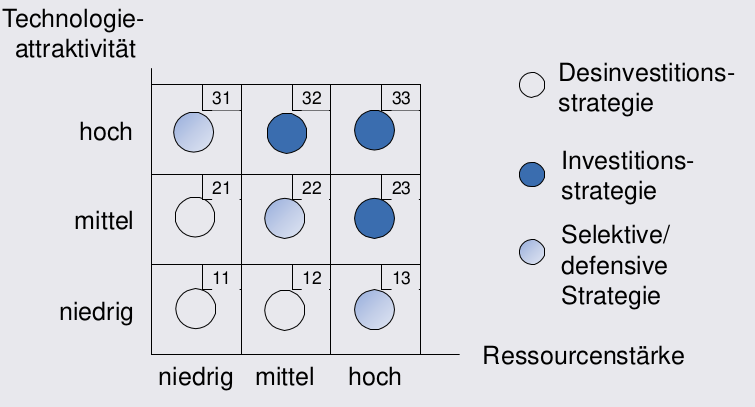
\includegraphics[width=250px]{./pictures/intechpo.png}
\caption{Technologie-Portfolio}
\end{figure} 

\begin{figure}[htbp]
\centering
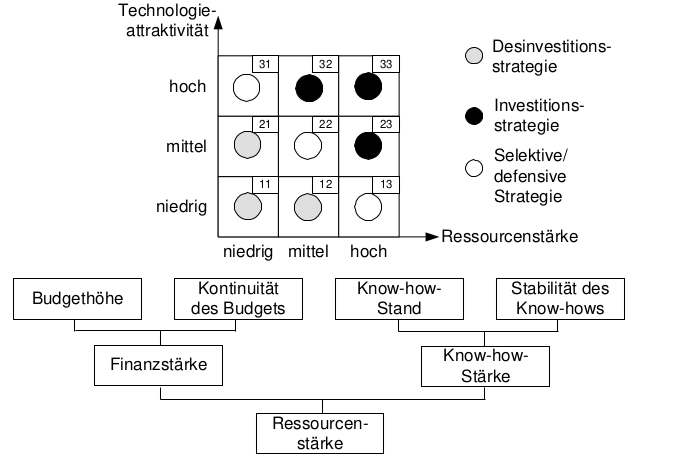
\includegraphics[width=250px]{./pictures/inrespo.png}
\caption{Ressourcenstärke \& Technologie-Portfolio}
\end{figure} 

\begin{enumerate}
\item Methoden technologischer Frühaufklärung
\label{sec:org2e826a9}
\begin{figure}[htbp]
\centering
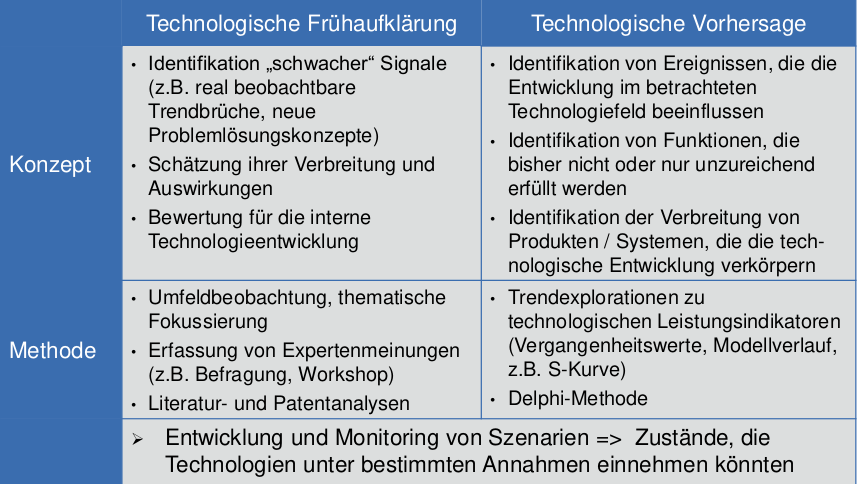
\includegraphics[width=250px]{./pictures/invor.png}
\caption{Frühaufklärung \& Vorhersage}
\end{figure}
\end{enumerate}

\subsubsection{Sicherung des Innovationswissens}
\label{sec:orge4e9e02}
\begin{figure}[htbp]
\centering
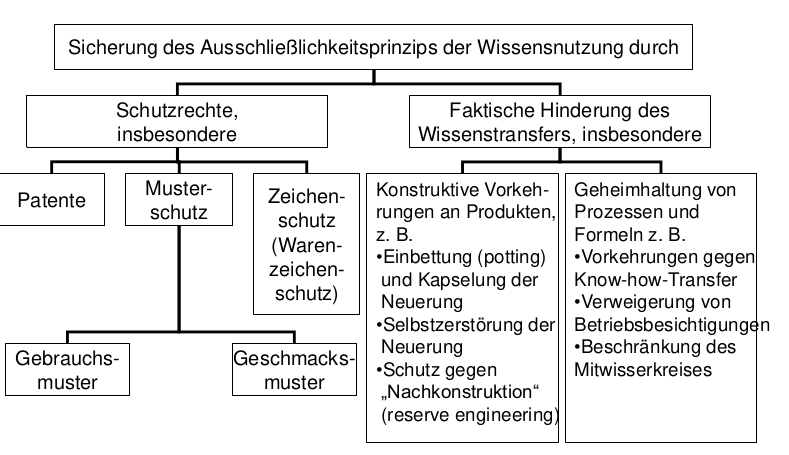
\includegraphics[width=250px]{./pictures/inauss.png}
\caption{Auschließlichkeitsprinzip zur Planung der Sicherung des Innovationswissens}
\end{figure} 

\begin{figure}[htbp]
\centering
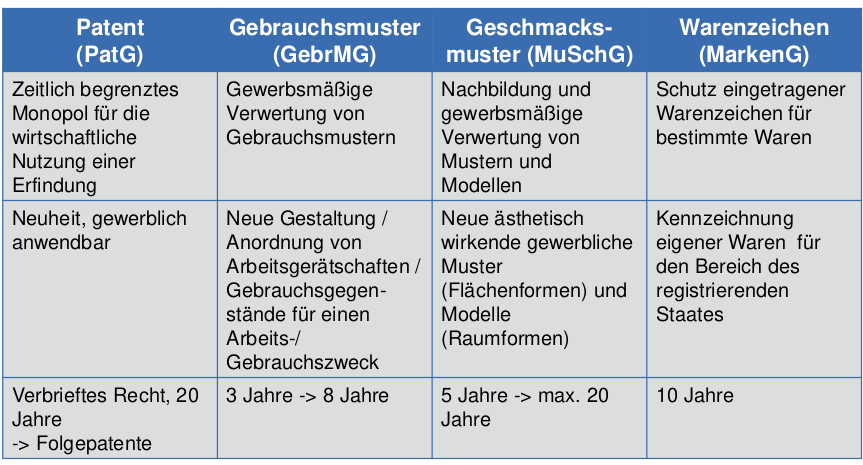
\includegraphics[width=250px]{./pictures/inmiss.png}
\caption{Rechtlicher Missbrauchsschutz}
\end{figure} 

IV\(_{\text{Innovationsmanagment}}\)\(_{\text{3.pdf}}\) F 17 Zsmfassung
\subsection{Innovationsprozesse als Managementaufgabe}
\label{sec:org4d286a0}
\begin{itemize}
\item nicht klausurrelevant
\end{itemize}
\end{document}
